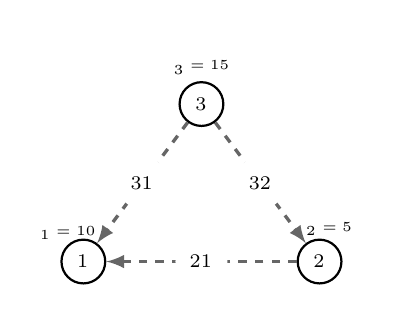
\begin{tikzpicture}[> = latex]
	\begin{scope}[every node/.style={circle,thick,draw}]%,label distance=-3px}]
		\node (a1)[label={[shift={(-0.2,-0.45)}]\tiny $\baseCosts_1 = 10$}] at (0,0) {$\feature_{1}$};
		\node (a2)[label={[shift={(0.12,-0.35)}]\tiny $\baseCosts_2 = 5$}] at (3,0) {$\feature_{2}$};
		\node (a3)[label={[shift={(0.0,-0.35)}]\tiny $\baseCosts_3 = 15$}] at (1.5,2) {$\feature_{3}$};
% 		\node (a1)[label={[shift={(-0.2,-0.45)}]\tiny $\baseCosts_1 = 10$}] at (0,0) {$\feature_{\texttt{Job}}$};
% 		\node (a2)[label={[shift={(0.12,-0.35)}]\tiny $\baseCosts_2 = 5$}] at (3,0) {$\feature_{\texttt{Edu}}$};
% 		\node (a3)[label={[shift={(0.0,-0.35)}]\tiny $\baseCosts_3 = 15$}] at (1.5,2) {$\feature_{\texttt{Loc}}$};
	\end{scope}

	\begin{scope}[
		every node/.style={fill=white,circle},
		every edge/.style={draw=black!60,dashed,very thick}]
		
% 		\path[->] (a1) edge[bend left=30] node {\small $\transition_{12}$} (a2);
		\path[->] (a3) edge node[] { $\transition_{32}$} (a2);
		\path[->] (a2) edge node[] { $\transition_{21}$} (a1);
		\path[->] (a3) edge node[] { $\transition_{31}$} (a1);
	\end{scope}
	
	
% 	\begin{sope}
% 	   % \node (1) at (1.0,2.7) {\scriptsize $\baseCosts_3 = $};
% 	   % \node (2) at (-0.1,1.02) {\scriptsize $\consequentialCosts_{1}(e_{31}) = $};
% 	\end{sope}
\end{tikzpicture}